% set home directory
\providecommand{\homedir}{..} 
% load the preamble of main.tex by subfiles
\documentclass[\homedir/main.tex]{subfiles}
% ##############################################################################
\begin{document}
% set chapter numbering to work correctly even when separate compilation using subfile
\setcounter{chapter}{3}
% ##############################################################################
\chapter{提案手法}\label{chap:methods}
本章では,まず\cref{sec:process_flow}で提案手法の処理の流れを説明する.
次に,\cref{sec:target_design_text}で対象とするデザイン文字列を明示する.
本章の最後に,\cref{sec:implementation}で\cref{sec:process_flow}で述べた処理の実装について述べる.

% ##############################################################################
\section{デザイン文字列を自動作成する処理の流れ}\label{sec:process_flow}
本手法では,次の\cref{fig:process_flow}のようにしてデザイン文字列を自動作成する.

\begin{figure}[h]
    \centering
    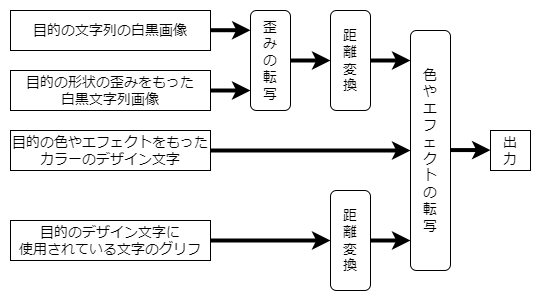
\includegraphics[keepaspectratio, width=0.8\linewidth]{process_flow.png}
    \caption{デザイン文字列の自動作成処理の流れ}
    \label{fig:process_flow}
\end{figure}

\cref{fig:process_flow}に示した処理の流れを順に説明する.

本手法を用いてデザイン文字列を作成するために必要な入力データは次の4つである.

\begin{enumerate}[label=\textbf{入力\arabic*:}]
    \item 出力されるデザイン文字列において使用したい文字列の白黒画像
    \item 出力されるデザイン文字列全体の形状の歪みを指定するための白黒文字列画像
    \item 出力されるデザイン文字列の色やエフェクトを指定するためのカラーのデザイン文字
    \item 入力3のカラーのデザイン文字に使用されている文字のグリフ
\end{enumerate}

これらのうち,まずは入力2のもつ形状の歪みを分析して入力1に形状の歪みを転写することで,
目的の形状の歪みを持った目的の文字列の白黒画像を作成する.
次に,形状の歪みの転写を用いて作成した白黒文字列画像と,入力4に対してそれぞれ距離変換を施す.
最後に,得た二枚の距離変換画像と入力3から最終的に出力するデザイン文字列を作成する.
以上が,本手法におけるデザイン文字列の自動作成処理の流れである.

% ##############################################################################
\section{対象のデザイン文字列}\label{sec:target_design_text}
本手法では,デザイン文字列のうち文字の配置が横一行のもののみを対象とする.
つまり,\cref{sec:background}で述べたようなデザイン文字列に特有のスタイルのうち,
文字列全体の形状の歪みのみを本手法の対象とし,文字の配置や文字の間隔などは対象外とする.

但し,形状の歪みによって文字配置が横一直線でなくなったものも本手法の対象とする.
例えば,次の\cref{fig:warp_and_place}の文字配置は傾いているが,
こうした文字列も本手法の対象とする.

\begin{figure}[h]
    \centering
    
\includegraphics[keepaspectratio, width=0.8\linewidth]{warp_and_place.png}
    \caption{デザイン文字列の自動作成処理の流れ}
    \label{fig:warp_and_place}
\end{figure}

\newpage
さらに,本手法での歪みの転写の実装上,入力2は次の二つの条件を満たす必要がある.

\begin{enumerate}[label=\textbf{条件\arabic*:}]
    \item 画像中の適切な位置で,適切な回数だけ,縦線で左右に画像を分割すれば,
          分割された各領域内の形状の歪みは単純な射影変換で再現できる.
    \item 条件1で述べた適切な画像の分割回数が文字数に比べて十分少ない.
\end{enumerate}

二つの条件のうち,条件1は目的とする形状の歪みが
射影変換を用いて再現可能であるための必要条件を表している.
例えば,次の\cref{fig:impossible_warp_style}の文字列は
いくら画像を縦線で左右に分割したとしても,
分割された各領域内の形状の歪みは単純な射影変換では再現できないため,本手法の対象ではない.

\begin{figure}[h]
    \centering
    
\includegraphics[keepaspectratio, width=0.8\linewidth]{impossible_warp_style.png}
    \caption{本手法の対象ではない形状の歪みをもった文字列画像の例}
    \label{fig:impossible_warp_style}
\end{figure}

一方,次の\cref{fig:poss_warp_wo_guide}の文字列は
画像の中央を通る縦線(\cref{fig:poss_warp_with_guide}の赤線)で左右に画像を分割すると,
分割された各領域内の形状の歪みが単純な射影変換で再現できるため,本手法の対象となる.

\begin{figure}[h]
    \centering
    \begin{minipage}[b]{0.45\linewidth}
        \centering
        
\includegraphics[keepaspectratio, width=0.95\linewidth]{possible_warp_style_without_guide.png}
        \subcaption{補助線なし}
        \label{fig:poss_warp_wo_guide}
    \end{minipage}
    \begin{minipage}[b]{0.45\linewidth}
        \centering
        
\includegraphics[keepaspectratio, width=0.9\linewidth]{possible_warp_style_with_guide.png}
        \subcaption{補助線あり}
        \label{fig:poss_warp_with_guide}
    \end{minipage}
    \caption{本手法の対象の形状の歪みをもった文字列画像の例}
    \label{fig:possible_warp_style}
\end{figure}

また,二つの条件のうち条件2は,
本手法において目的とする形状の歪み方がうまく検出されるために必要な条件を表している.
(後の\cref{sec:warp_style_transfer}で詳述する.)

% ##############################################################################
\section{実装}\label{sec:implementation}
\subsection{文字列の歪みの転写}\label{sec:warp_style_transfer}
\cref{sec:process_flow}で述べた処理のうち,文字列の歪みの転写は次のように行っている.

バウンディングボックスの検出

歪みの数を決定する(後述)

区分線形回帰

歪みの数の決定方法

制御点の位置を計算

\begin{algorithm}[h]
    \caption{文字列の歪みの転写}
    \label{alg-X}
    \begin{algorithmic}[1]

        \Function {max\_in\_array}{$array$}
        \State $max \gets 0$
        \ForAll {$element \gets array$}
        \If {$element > max$}
        \State $max \gets element$
        \EndIf
        \EndFor
        \State \Return $max$
        \EndFunction

    \end{algorithmic}
\end{algorithm}

\subsection{距離変換および色やエフェクトの転写}
先行研究\cref{X}で提案されたモデルを用いる.



% ##############################################################################
\printBibForSubfiles
\end{document}